\chapter{Functional testing}

\section{Introduction}

Our first task is to check the functional correctness of the application. The functional tests to be carried out are:
\begin{enumerate}
 \item Check each application configuration for the occurence of Java exceptions;
 \item Check each application configuration for any aggressive memory leaks i.e. any leaks that would cause the JVM to run out of memory if the application was left running.
\end{enumerate}

Any configurations that exhibit any of the above behaviour\footnote{an application 'fault'} will be discounted from any further performance testing. As far as the black-box methods that are available to us allow, we will investigate the extent and location of the fault.

\section{Exceptions}

\subsection{Method}

To check for occurrence of Java exceptions in our application we set up our application with some added monitoring. We used a profiler tool\footnote{see appendices} that carried out instrumentation of specified classes (in our case those in package org.adaptivecellsj). The trace files produced by this tool gave us the calling sequence for these instrumented classes, enabling us to identify the bean that raised the exception (in conjunction with the diagram in figure \ref{fig_bean_calling}. From the AdaptiveCells/J documentation we know that each bean calls a method, 'simulateBusinessLogic', we can see during which particular call to this method the exception is raised, thus identifying the bean e.g. if for config1 the exception is raised in the second call to simulateBusinessLogic then the bean that raised the exception is TB2.

We invoked each configuration, in sequence, through the web page front end, accessible at url http://localhost:8080/adaptivecellsj/start.html. If an exception was raised we examined the JBoss log, and the trace file produced by the profiling tool.

\subsection{Results}

We established that three configurations raised exceptions\footnote{all of type java.lang.RuntimeException} config4, config5. Nothing of note was observed in the JBoss logs. Examination of the trace files showed that the following:

\begin{center}
\begin{tabular}{| c | c |}
 \hline
 Config & Bean raising exception \\
 \hline
 config4 & TB5 \\
 config5 & TB4 \\
 \hline
\end{tabular}
\end{center}

We repeated the test to check our results, which confirmed our initial findings. We can now discount config4, config5 from further testing.

\section{Memory Leaks}

\subsection{Method}

Despite Java having garbage collection memory leaks can still occur, primarily where an object is put into a long lived collection and not taken out once the object is no longer required.

The instructions for the assignment state that we identify aggressive memory leaks and remove them from further investigation. For our purposes we define an aggressive memory leak as one that would result in heap exhaustion within standard use of the application i.e. the memory is not freed by garbage collection.

We know from the AdaptiveCells/J documentation that memory leaks are implemented by allocating an array of bytes. Any aggressive memory leak should be visible as a large block of memory that isn't freed after a garbage collection. To identify configurations with aggressive memory leaks we used the following method:

\begin{enumerate}
 \item Monitor the application with JConsole;
 \item Using JMeter to create workload for 100 users access to AdaptiveCells/J at the same time;
 \item Setting up the loopcount in JMeter is forever in 60 minutes;
 \item Invoke the AdaptiveCells/J configuration that we are currently investigating, and then take a snapshot of memory usage;
\end{enumerate}

The above method was repeated for each of the configurations that did not cause Java exceptions to be raised. An aggressive memory leak should be evident from observing a steady increase in the memory allocated to byte arrays and that this allocation should not significantly decrease following the forced garbage collection.

\subsection{Results}

After testing each configuration for one hour, we found three configs cause memory leak including: config1, config2, and config9. Normally, garbage collection mechanism of Java will collect memory of system after used. The graph of the used memory continually fluctuated in the operation time of the system. Figure \ref{config3} showed the normal operation of the system. 

\begin{figure}[ht]
 \centering
 \scalebox{0.45}{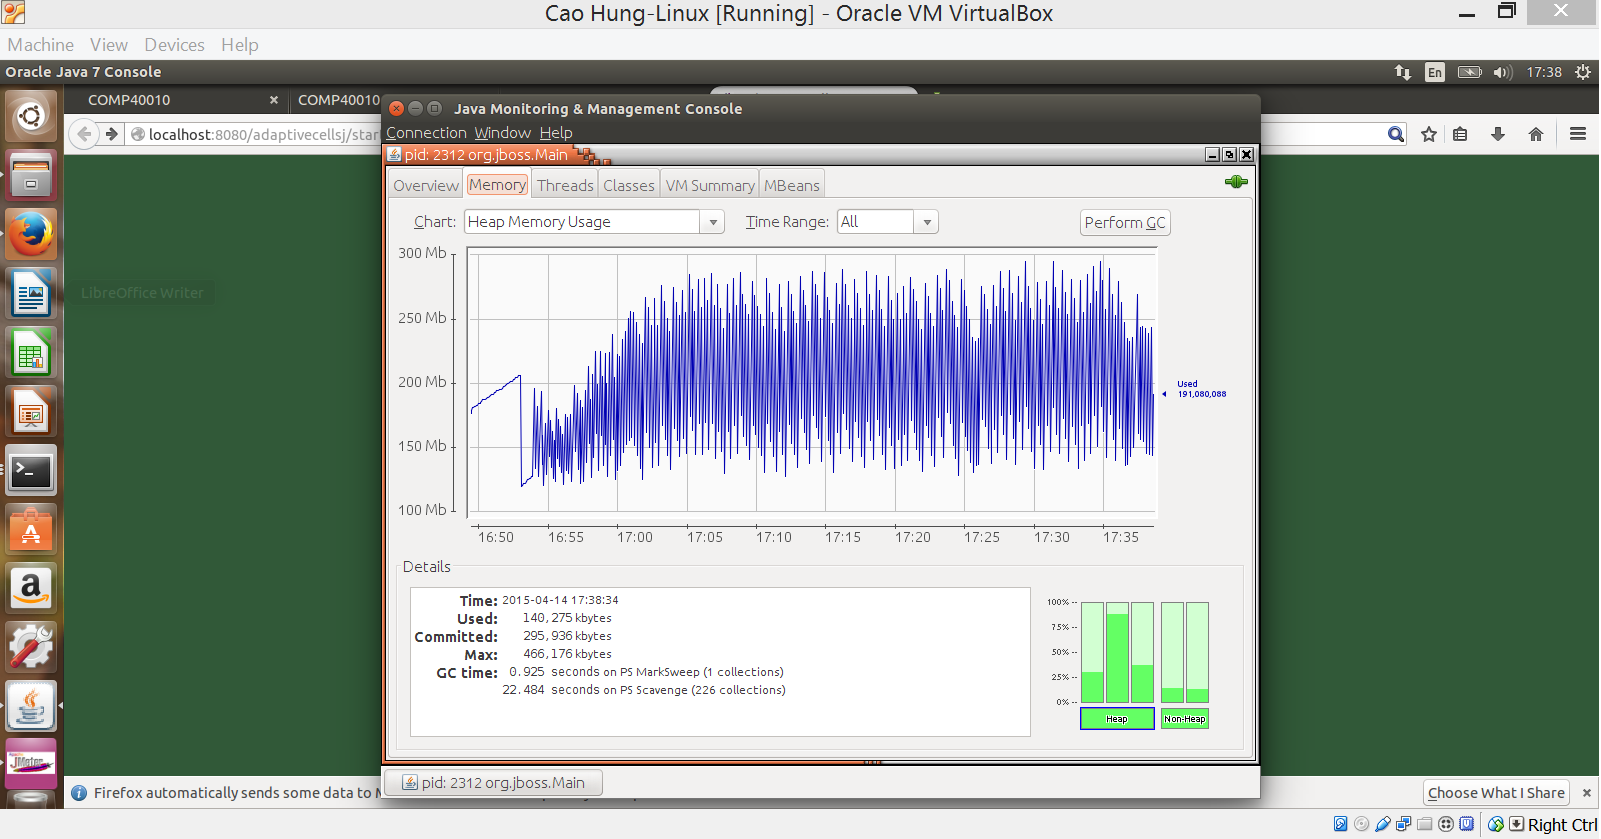
\includegraphics{Graphics/config3.png}}
 % func_memory_leaks.png: 638x448 pixel, 72dpi, 22.51x15.80 cm, bb=0 0 638 448
 \caption{Graph showing normal work of config 3}
 \label{config3}
\end{figure}

However, when memory leak occur in the system, the garbage collection mechanism could not free all memory and some spaces of memory was still occupied. After a certain time, the memory leak climbed higher and higher until the system absolutely crashed. An example of this case was indicated in Figure  \ref{config2}.

\begin{figure}[ht]
 \centering
 \scalebox{0.5}{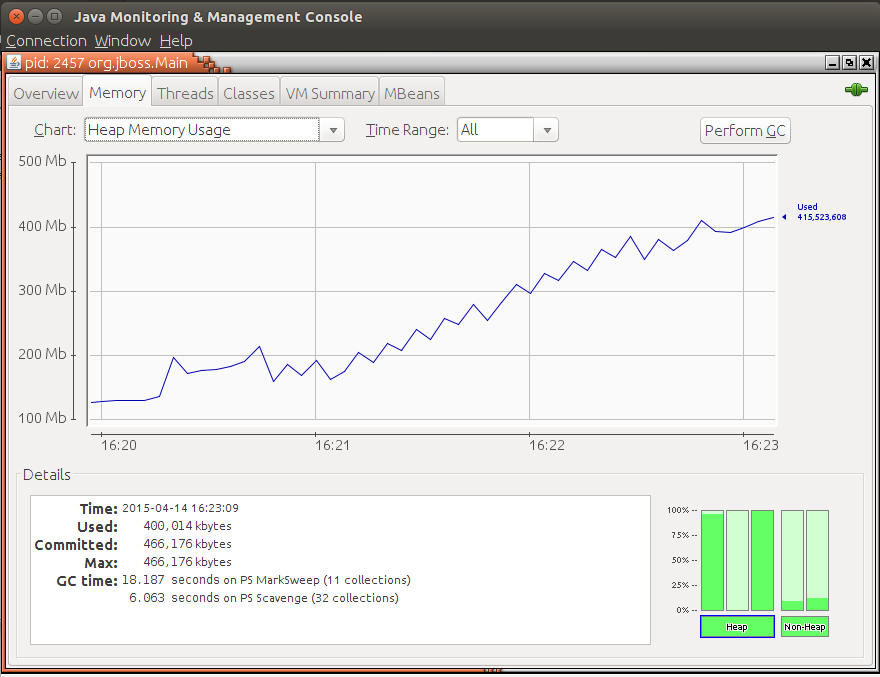
\includegraphics{Graphics/config2.png}}
 % func_memory_leaks.png: 638x448 pixel, 72dpi, 22.51x15.80 cm, bb=0 0 638 448
 \caption{Graph showing memory leak situation was caused by config 2}
 \label{config2}
\end{figure}

We established that two configurations had aggressive memory leaks, config1, config2 and config9. Table \ref{func_mem_leak_table} shows the data obtained.

\begin{figure}[h]
 \centering
\begin{tabular}{| c | c | c | c |}
 \hline
  & \multicolumn{3}{|c|}{Config} \\ \cline{2-4}
 Stage & config1 & config2 & config9\\
 \hline
 before running & 120,703,904 & 125,034,504 & 125,034,504 \\
 after collapse & 410,528,952 & 415,523,608 & 415,565,984 \\
 \hline
\end{tabular}
 \caption{Change in memory (from initial reading) allocated to byte[]}
 \label{func_mem_leak_table}
\end{figure}

Figure \ref{config2_2} indicated the error when the system collapse by the memory leak.

\begin{figure}[ht]
 \centering
 \scalebox{0.45}{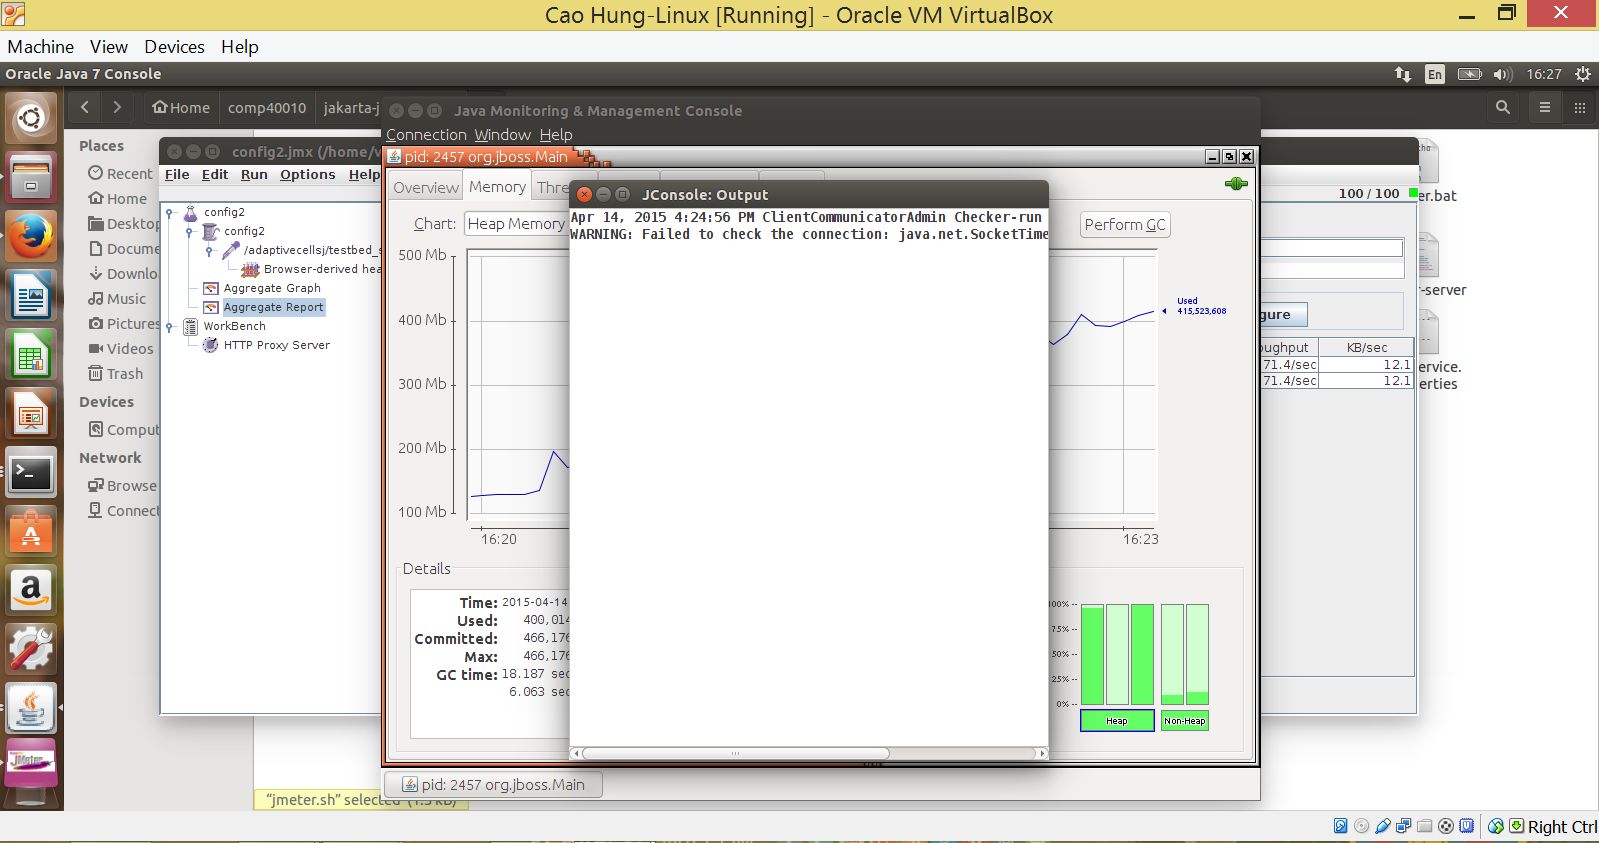
\includegraphics{Graphics/config2_2.png}}
 % func_memory_leaks.png: 638x448 pixel, 72dpi, 22.51x15.80 cm, bb=0 0 638 448
 \caption{Error when memory leakage happened}
 \label{config2_2}
\end{figure}

\section{Summary}

Following our functional testing we can discount config1, config2, and config9 because of agressive memory leaks and config4, config5 because of raising Java exceptions. This leaves config3, config6, config7, config8, and config10 remaining to carry out performance analysis on.